\section{Functionnal Architecture}

\subsection{Introduction}
The functionnal architecture constitutes the specifications of the project and allows us to have criteria
for the success of our project. \textbf{Figure}~\ref{fig:requirement} shows us the requirements
diagram that follows the \textit{SysML} standard for this system.

\begin{figure}[!ht]
    \begin{center}
        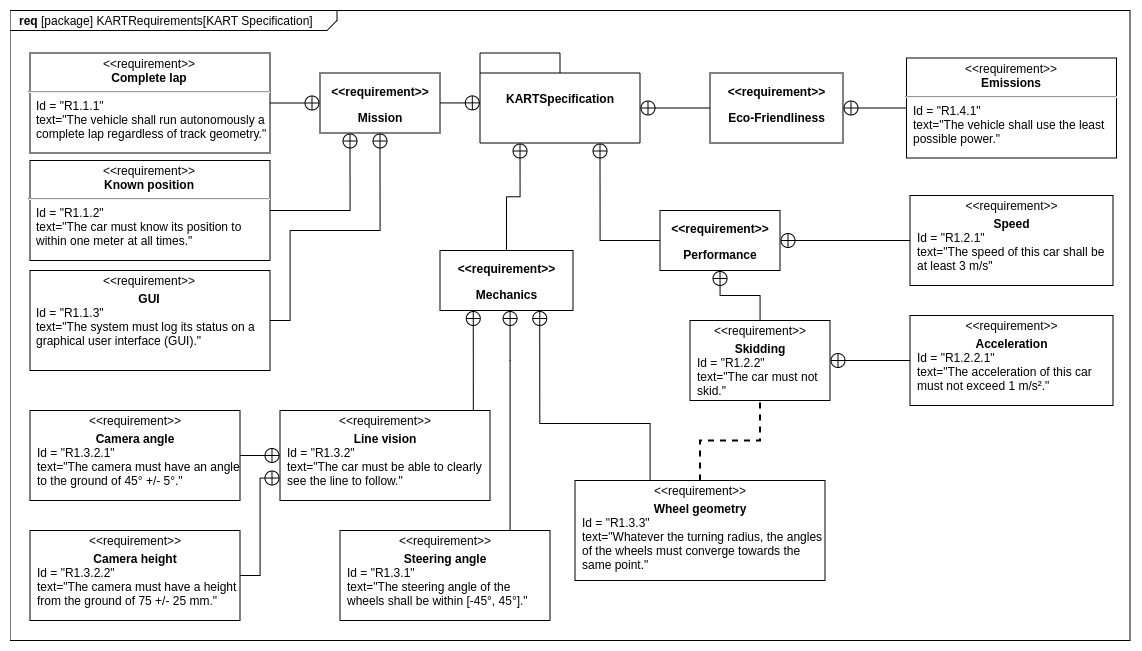
\includegraphics[width=\textwidth]{Images/requirement.png}
    \end{center}
    \caption{Functionnal Architecture of this project}
    \label{fig:requirement}
\end{figure}

The requirements diagram in \textbf{Figure} \ref{fig:requirement} shows us the requirements we want for this system. The requirements are divided into several categories.

First there is a mission requirement that the robot must follow. It must therefore know its position and be able to communicate it to the user through a graphical user interface. In addition, the car must perform laps around the track regardless of its shape.

Then we have requirements in terms of the mechanics and design of the robot. The car must not skid on the track under any circumstances, as this would lead to a loss of control of the track. In addition, there is a requirement for the camera to be positioned and oriented so that it can observe the line in the best possible conditions.

Then there are performance requirements, including a minimum speed to be respected, as the goal of the mission remains to complete laps of the track as quickly as possible. There is also a requirement for maximum acceleration, which will allow the car to remain in control of the car while avoiding loss of grip on the track.

Finally, as the system is an on-board system, it operates on battery power and therefore it must meet a criterion of resonant battery usage. It should be noted that by limiting the car's acceleration, the energy balance is much better and the battery is saved. This allows the system to work longer and in better conditions.

\newpage